%%=============================================================================
%% Methodologie
%%=============================================================================

\chapter{\IfLanguageName{dutch}{Methodologie}{Methodology}}%
\label{ch:methodologie}

%% TODO: Hoe ben je te werk gegaan? Verdeel je onderzoek in grote fasen, en
%% licht in elke fase toe welke stappen je gevolgd hebt. Verantwoord waarom je
%% op deze manier te werk gegaan bent. Je moet kunnen aantonen dat je de best
%% mogelijke manier toegepast hebt om een antwoord te vinden op de
%% onderzoeksvraag.
\section{Inleiding}

In dit onderdeel wordt de onderzoeksaanpak besproken. Dit zal een overzicht voorleggen van de  nodige stappen die ondernomen worden om de POC's en vergelijkende studie te realiseren.

Bij de start van het onderzoek wordt de eerste POC opgemaakt omdat hiervoor geen vereiste kennis nodig is over Three.js. Zo kan deze conventionele versie als een basis dienen voor de tweede POC. Beide POC's dienen zo identiek mogelijk te zijn waarbij het verschil ligt bij het implementeren van Three.js.

Het concept voor beide webshops is een online vinyl winkel, hierbij zal gebruik gemaakt worden van de Spotify API. Deze API zal voornamelijk benut worden om mockdata te voorzien. De keuze voor een vinyl webwinkel is omdat de 3D modellen die zullen gebruikt worden relatief simpel zijn.

De vergelijkende studie zal afgelegd worden m.b.v. UX metrics. Deze geven ons concrete metingen...

\section{Mock-ups}

Alvorens er een lijn code geschreven wordt zijn er mock-ups gemaakt voor de mobiele versie \ref{fig:mobileMockUps} en de desktop versie, beide voor de Home Pagina \ref{fig:desktopHomeMockUp} en de Detail Pagina \ref{fig:desktopDetailMockUp}. Zoals eerder vermeld dienen de mock-ups als een basis voor de conventionele versie van de webshop om een goede UX/UI te voorzien.

\begin{figure}
	\centering
	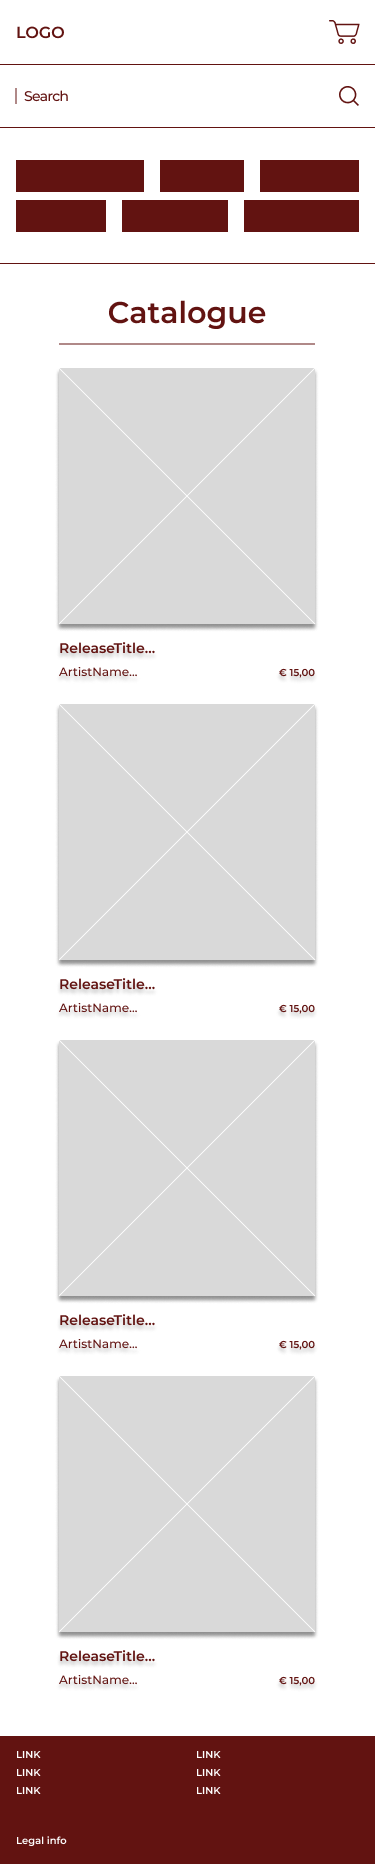
\includegraphics[width=0.3\linewidth]{graphics/HomePageMobile}
	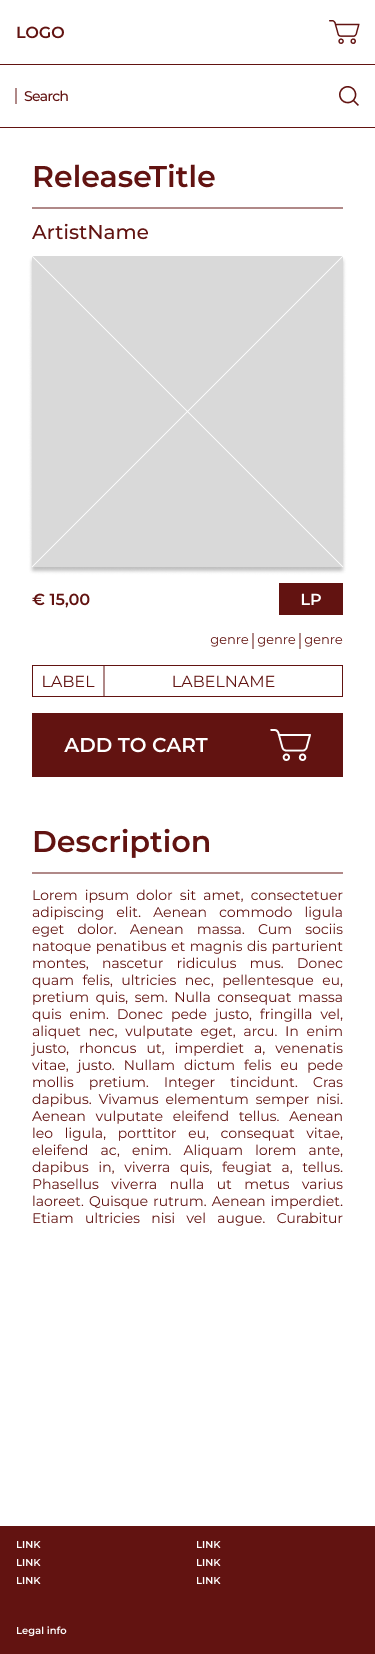
\includegraphics[width=0.3\linewidth]{graphics/DetailsPageMobile}
	\caption[Mock-Ups Mobile]{Mock-Ups Mobile}
	\label{fig:mobileMockUps}
\end{figure}

\begin{figure}
	\centering
	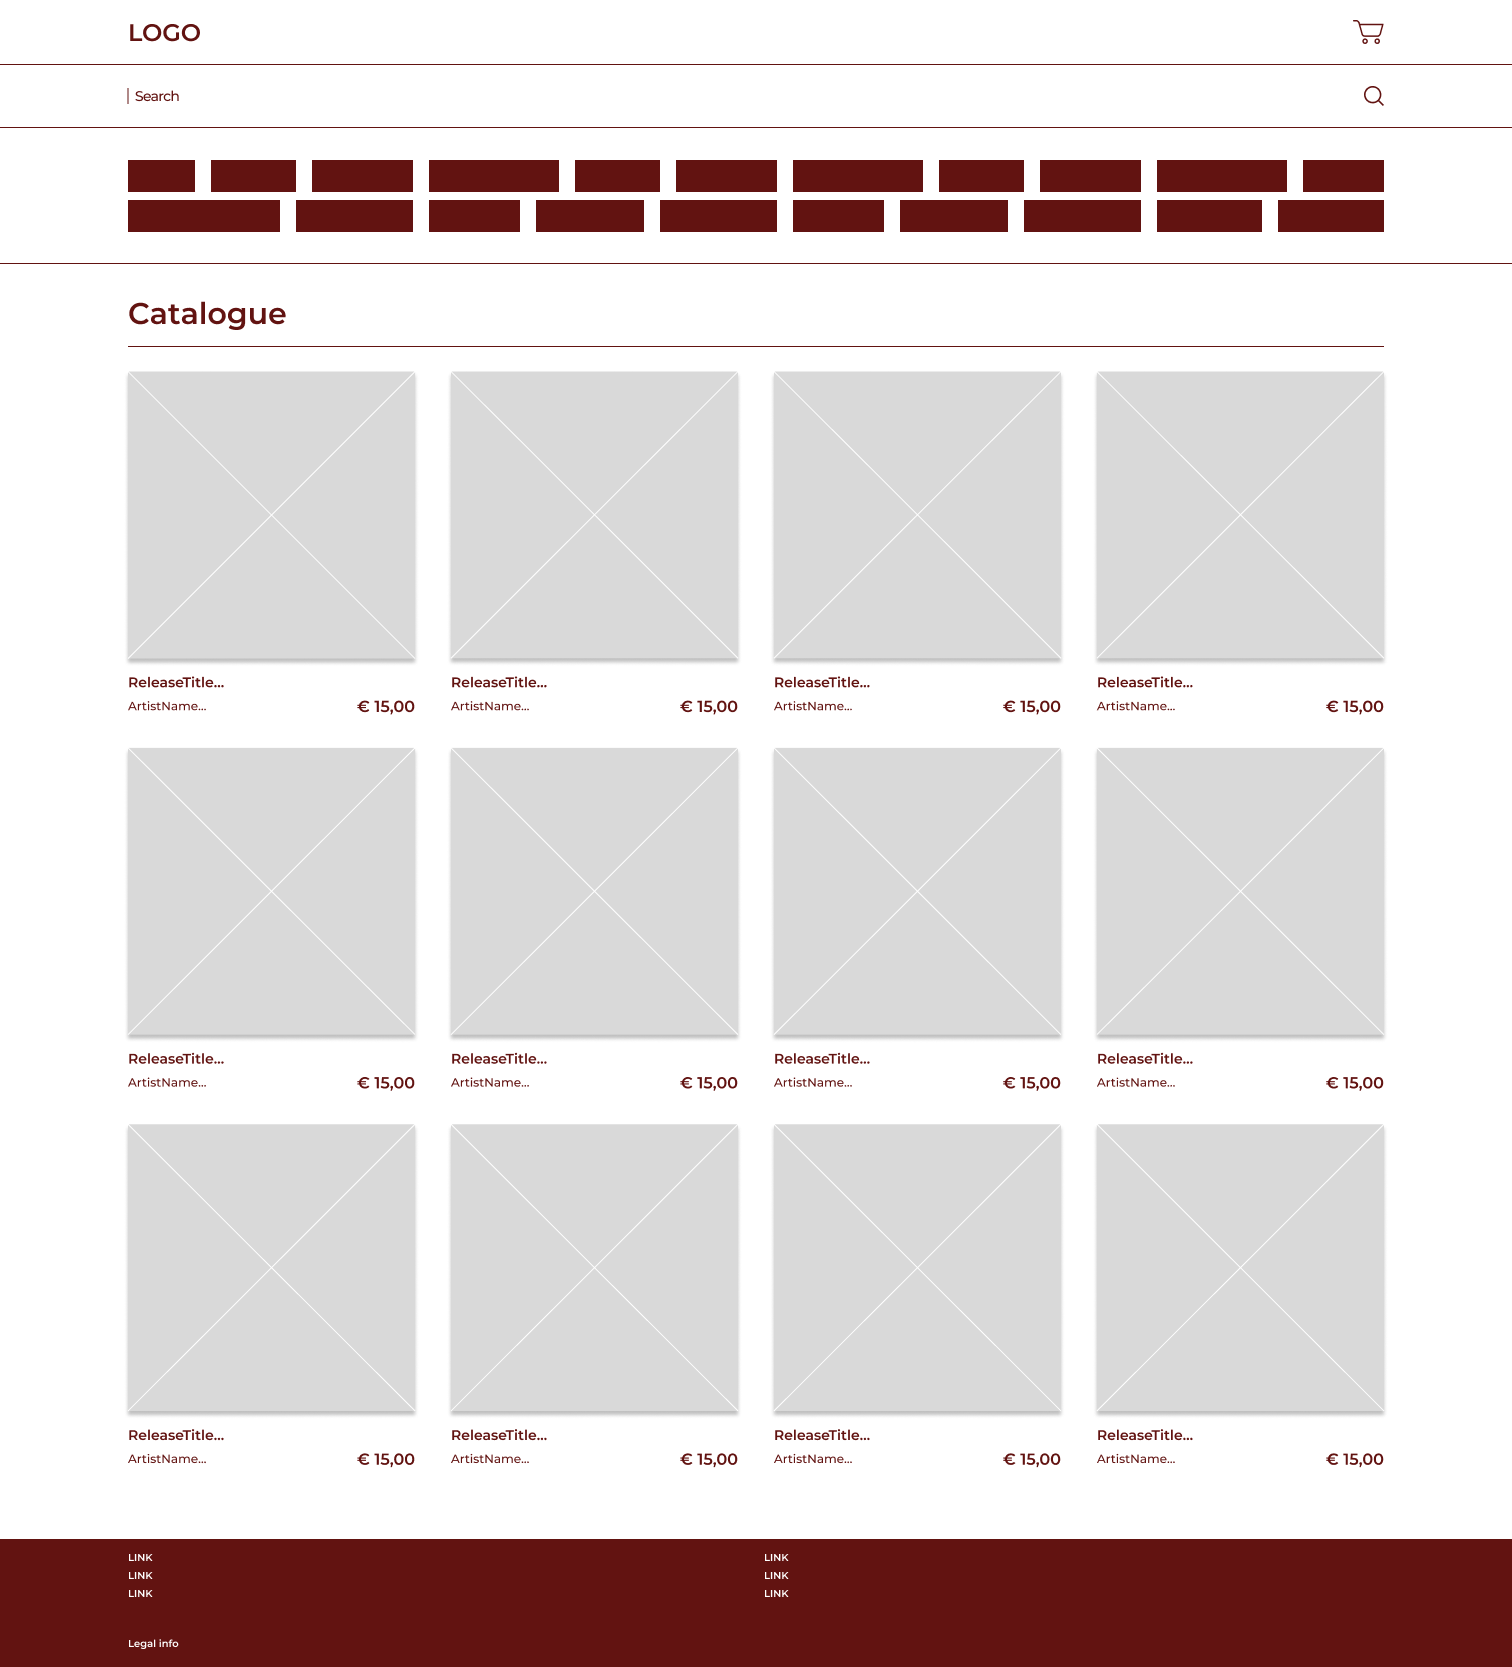
\includegraphics[width=1\linewidth]{graphics/HomePageDesktop}
	\caption[Mock-Up Desktop]{Mock-Up Desktop Home Pagina}
	\label{fig:desktopHomeMockUp}
\end{figure}

\begin{figure}
	\centering
	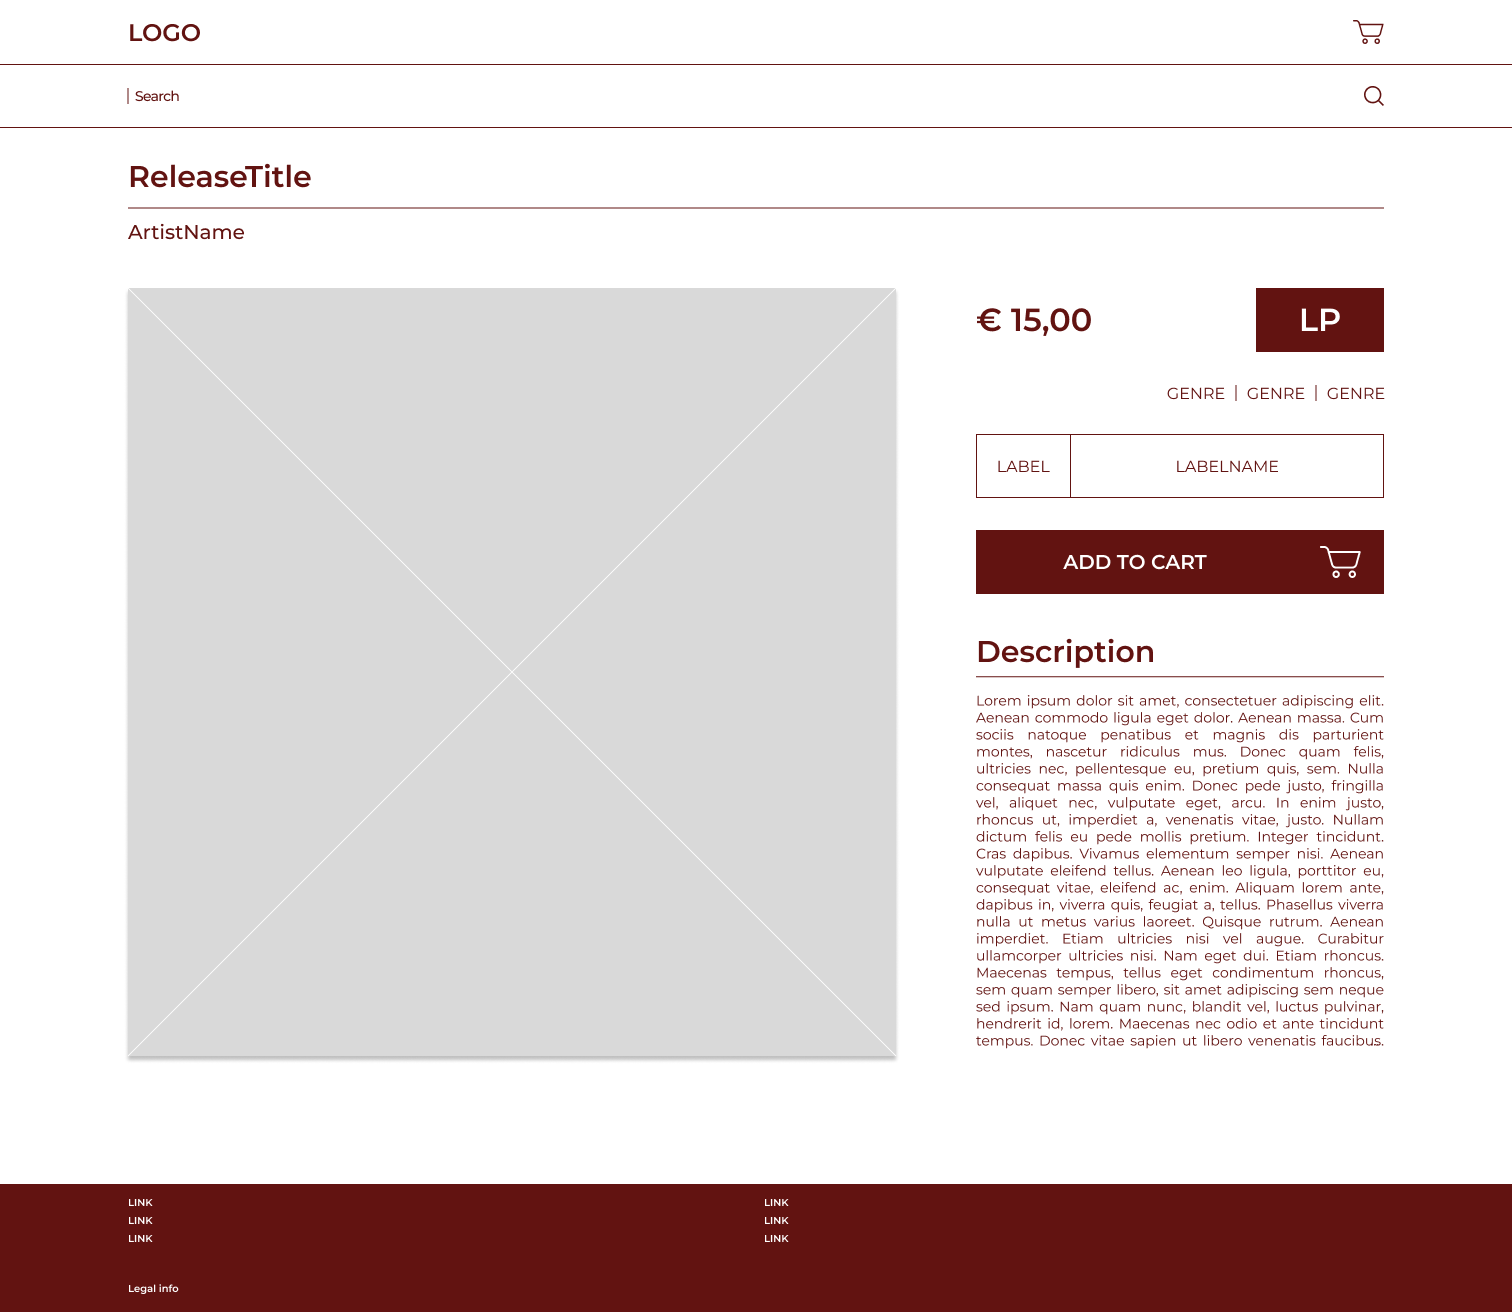
\includegraphics[width=1\linewidth]{graphics/DetailPageDesktop}
	\caption[Mock-Up Desktop]{Mock-Up Desktop Detail Pagina}
	\label{fig:desktopDetailMockUp}
\end{figure}

\pagebreak

\section{Proof-of-concept: Conventioneel}

De conventionele POC is de eerste die zal verwezenlijkt worden. Deze zal bestaan uit een React front-end en een Node.js backend om de Spotify API te hanteren. De reden voor het gebruiken van React en Node.js is omdat ze behoren tot de meest gebruikte frameworks voor het bouwen van websites.

Voor een goede flow te voorzien zijn een aantal user stories opgemaakt voor het concept van de vinyl webshop. Deze zijn:

\begin{itemize}
	\item Als Klant wil ik gemakkelijk navigeren door de selectie van vinyl op de webshop, filterende op artiest, album titel, etc., zodat ik de releases die ik wil snel kan terugvinden.
	\item Als Klant wil ik gedetailleerde informatie kunnen zien over elke release zodat ik een geïnformeerde beslissing kan maken of ik de release al dan niet zal kopen.
\end{itemize}

Om een degelijke webshop te realiseren worden eerst mockups gemaakt a.d.h.v. Figma. De reden hiervoor is omdat een goede UX/UI nodig is voor beide POC's. De inhoud en opbouw van deze POC wordt uitgebreid uitgelegd in volgend hoofdstuk~\ref{ch:proofofconceptConventioneel}

\section{Proof-of-concept: Three.js}

De POC die gebruik maakt van Three.js zal dus beginnen vanaf een kopie van de conventionele POC. Hierbij zullen een aantal aanpassingen gemaakt worden aan de webshop die van de technologie gebruik maken. Er wordt geprobeerd om zo dicht mogelijk te blijven bij de conventionele POC om een correcte vergelijkende studie uit te voeren.
